Building a toy model for derivation production jobs provides a schema by which it makes using real data and Monte Carlo simulated data much simpler.
One general principle about both data and Monte Carlo is the branch data within both is made up a mixture of randomized floats and repeated integer-like data.
Replicating this mixture of compressible/incompressible values in a branch would give us an effective model that would resemble how current derivation jobs would act on real or MC simulated data. 
These toy model TTree mixtures would provide a platform to test limiting basket sizes to see how it affects compression and how evident its effects may be. 

\section{Introducing the Toy Model}

The first toy model example that was investigated was filling up a TTree full of branches that have some amount of random floats saved.
The original conception was to first set up four distinct branches, each with a set number of events ($N=1000$), and each event having a number of entries, vectors with 1, 10, 100, and 1000 floats per vector.
Specifics are illustrated in Appendix \ref{appendix:toy_model_no_mix_code}.

\begin{figure}[h]\label{fig:toymodel_compF_rndm_vectors}
    \caption{Compression factors of $N=1000$ entries per branch with random-valued vectors of varying size.}
    \centering
    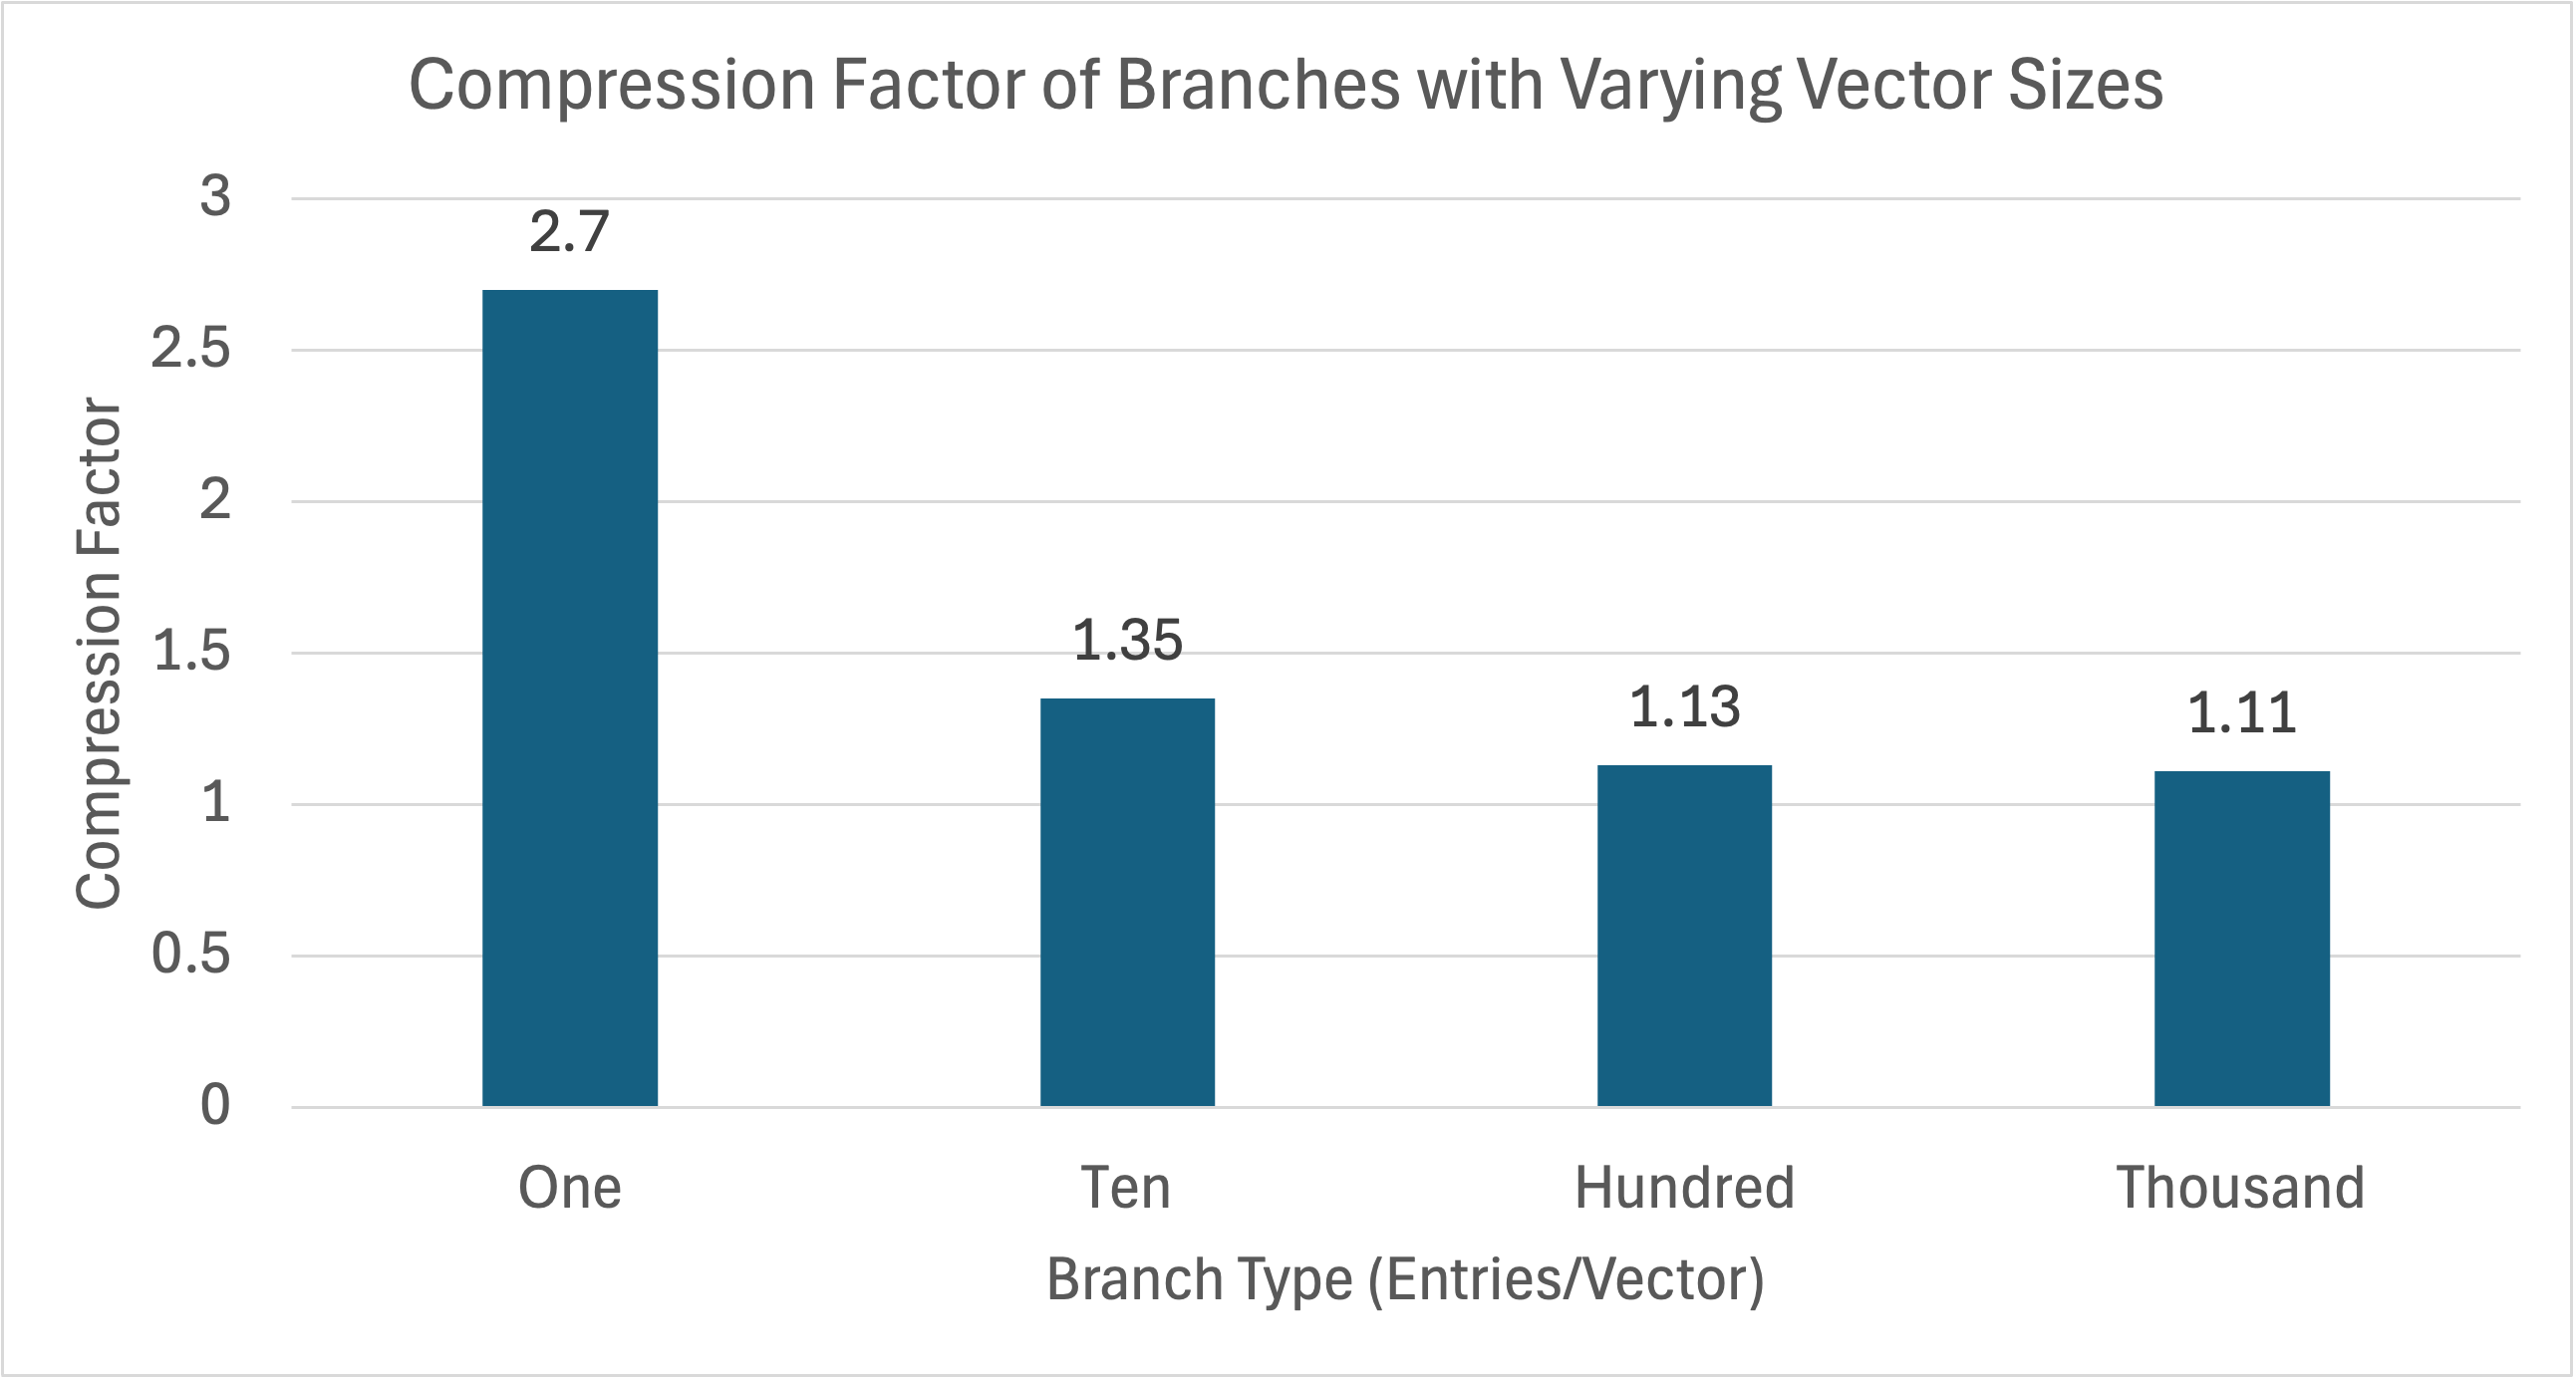
\includegraphics[width=.8\textwidth]{content/toymodel_content/branch_compfacts_nomix.png}
\end{figure}

What was of interest here was the compression factor for each branch that was filled. Results are shown in Figure \ref{fig:toymodel_compF_rndm_vectors}.
In this case, the smaller the branch, the less information to compress leading to higher compression in the smaller branch.
This outcome isn't going to yield results similar to data/MC type branches, Figure \ref{fig:toymodel_filesize_rndm_vectors}

\begin{figure}[h]\label{fig:toymodel_filesize_rndm_vectors}
    \caption{File size of $N=1000$ entries per branch with random-valued vectors of varying size.}
    \centering
    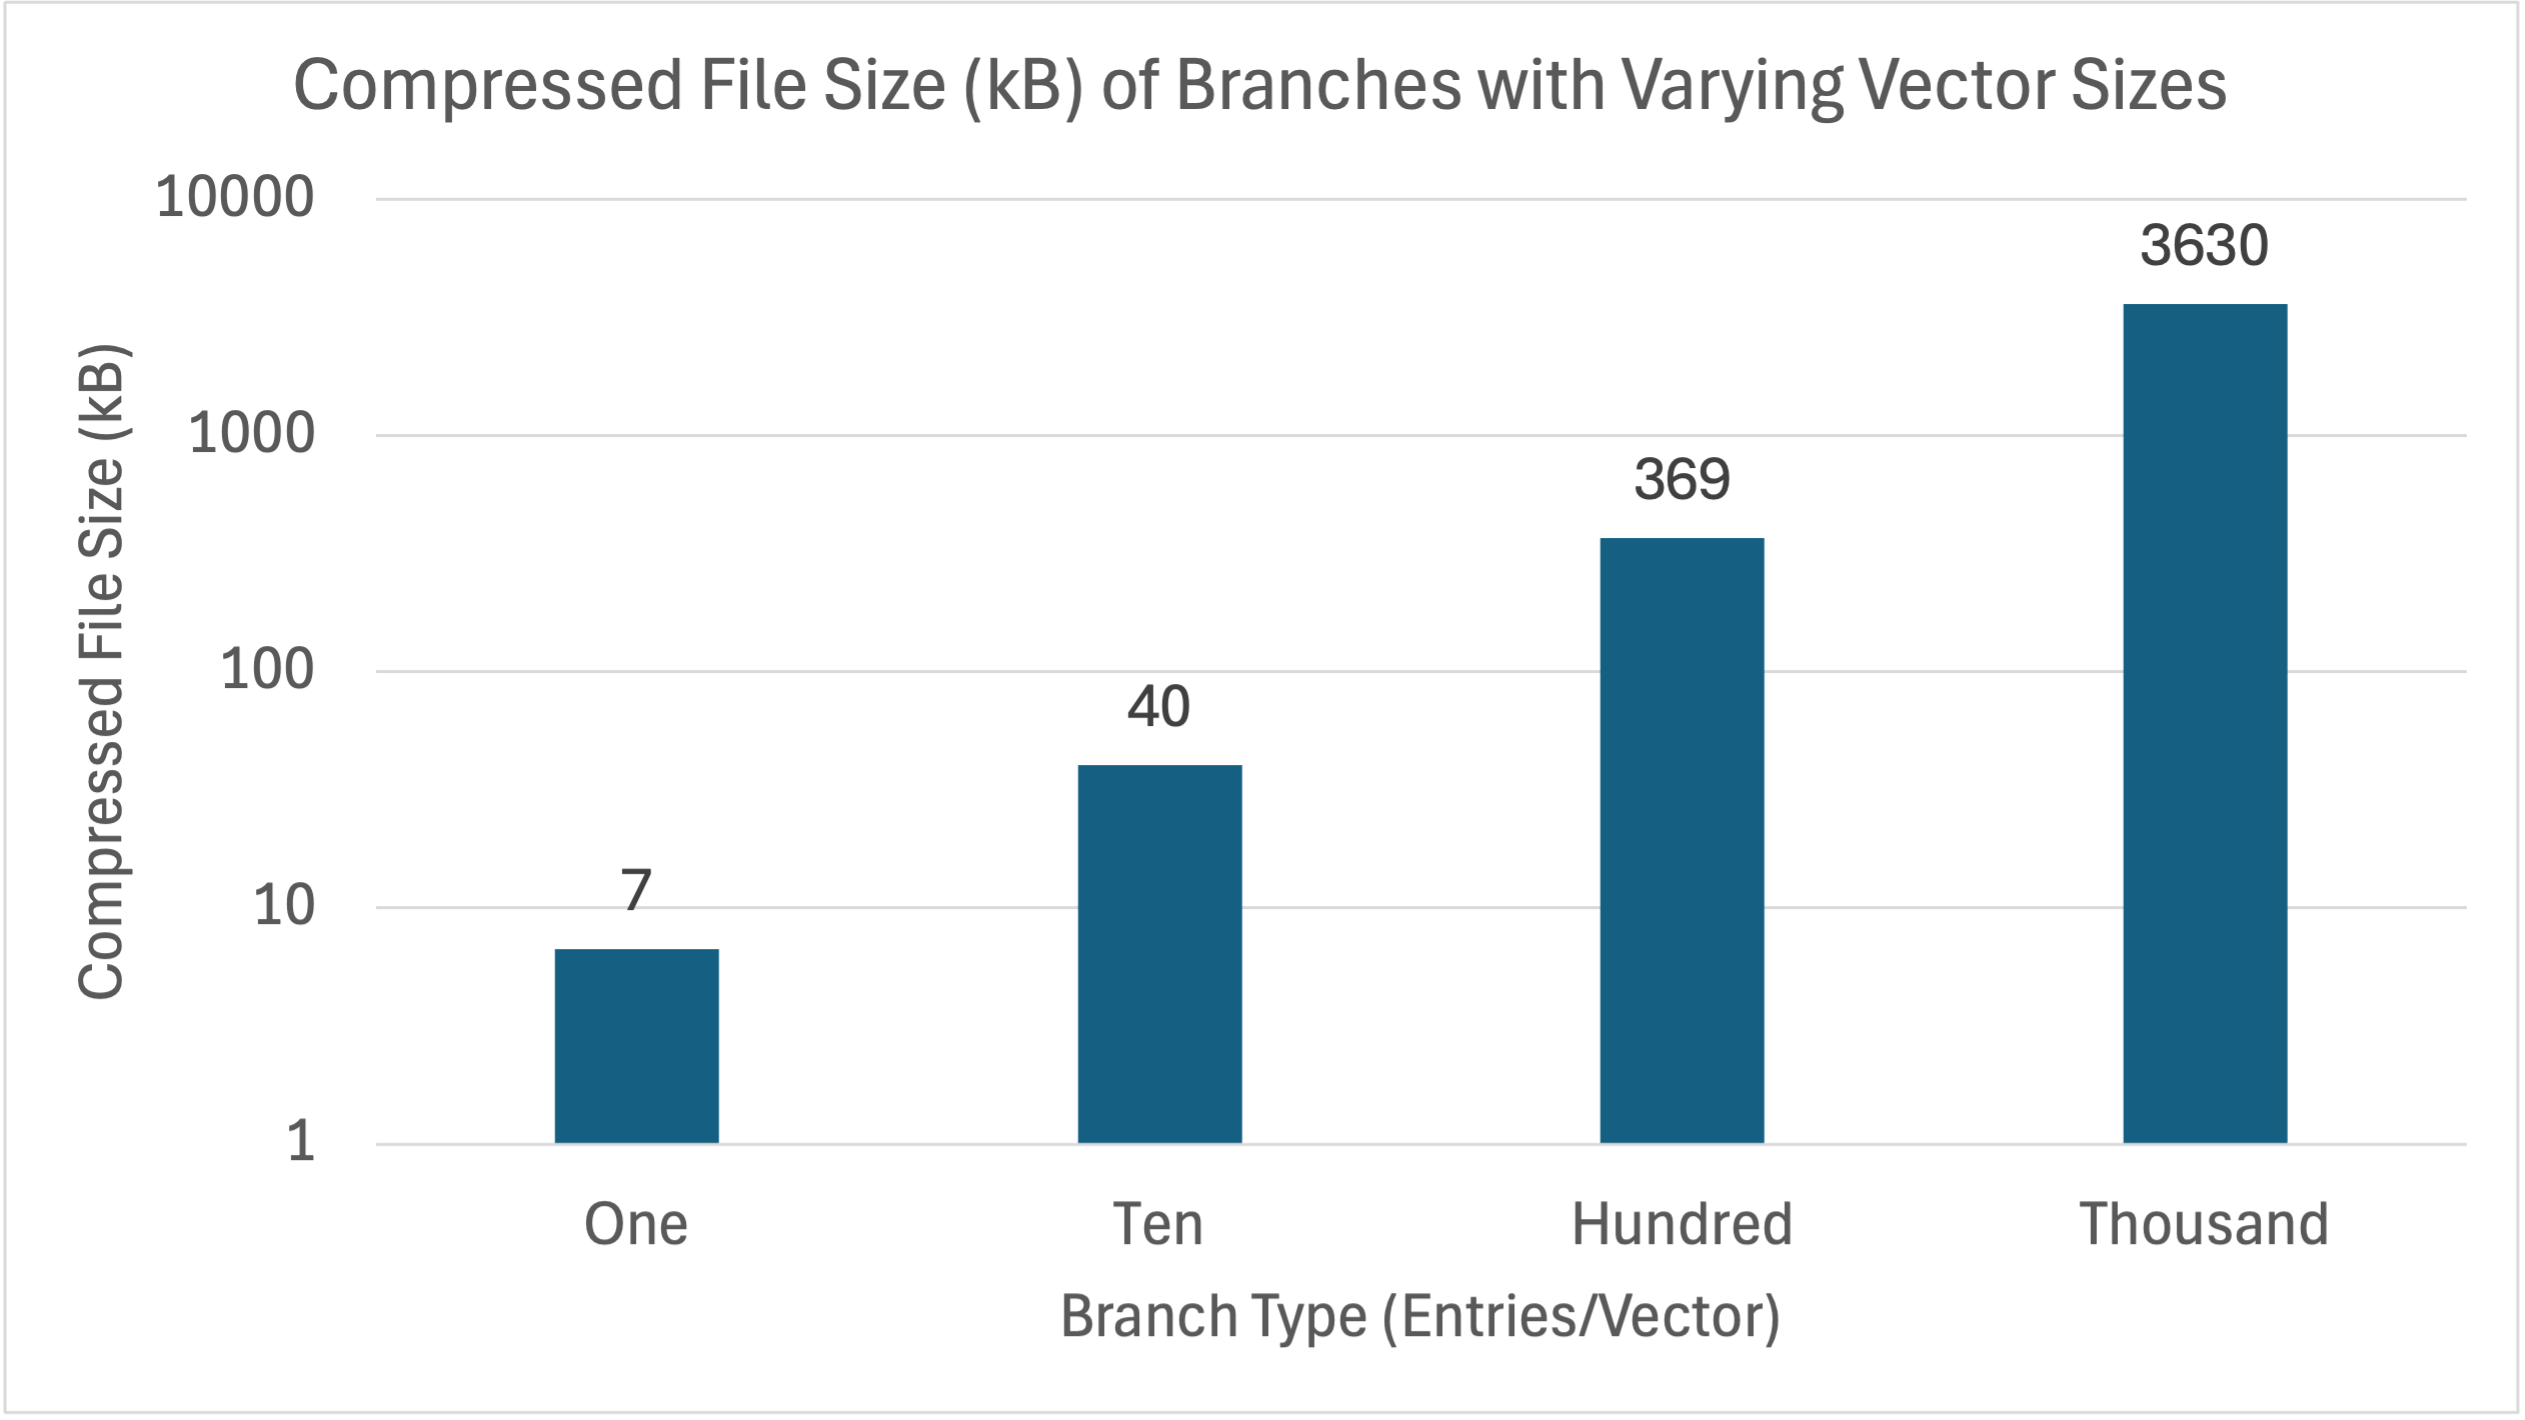
\includegraphics[width=.8\textwidth]{content/toymodel_content/branch_fileSize_nomix.png}
\end{figure}

After establishing  was possible to mix up each entry with a number of random-valued float values 

\section{Toy Model Derivation Production}

Once the toy model was sufficiently similar to what we would expect to see in real data/MC AODs, the next step was to run derivation production jobs. 
These jobs would take the input AODs that we filled with mixtures of random and non-random floats and compress them down. 

The focus at this stage of testing was on the compression factor when varying basket sizes. 